\section{}
\FloatBarrier
% 2) Hall-effect sensor
% a) Plot the data for the Hall-effect sensor to find the correlating function (i.e.
% displacement vs. voltage). As you can see from the data, the sensor is quite non-linear. In 
% such cases it's normal to use a polynomial correlating function to “linearize” the sensor. Fit 
% your data with a 3rd order polynomial. Report the equation used in the fit of your data. 
\subsection{}
\begin{figure}[h]
    \centering
    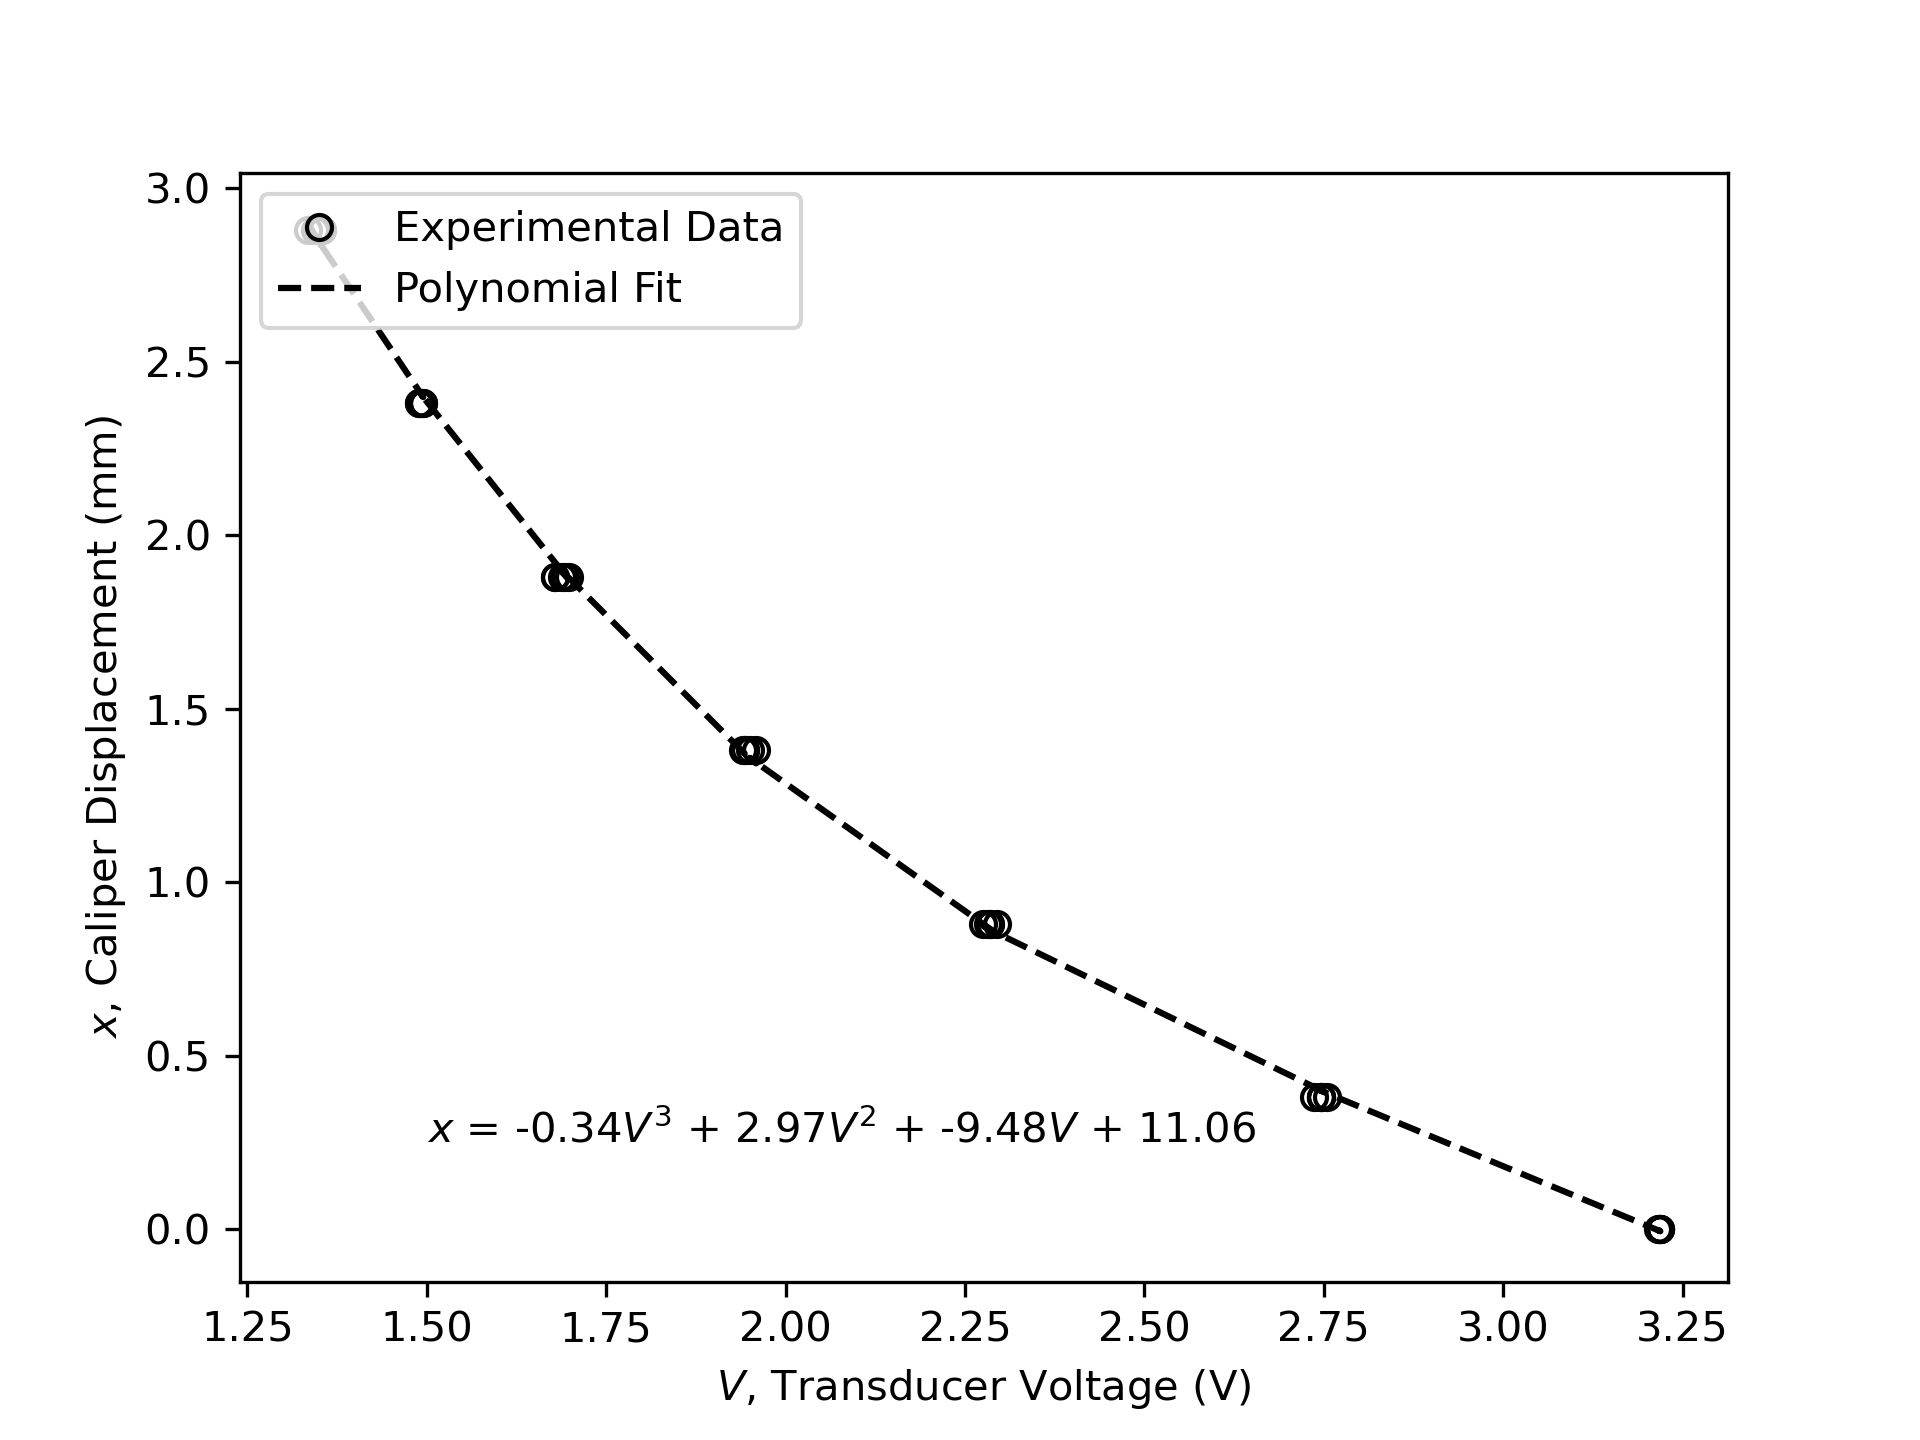
\includegraphics[width=0.8\linewidth]{matplotlib/Q2a.png}
    \caption{Hall-effect sensor data}
    \label{fig:Q2a}
\end{figure}

The coefficients of the polynomial of the form $y = ax^3 + bx^2 + cx + d$ were taken using the \texttt{=LINEST(x, y\string^\{1, 2, 3\}, True, True)} 
function in Excel. The coefficients are shown in Table \ref{tab:Q2a}.

\begin{table}[h]
    \centering
    \caption{Coefficients of third degree fitting polynomial for Hall-effect sensor measurements}
    \label{tab:Q2a}
    \begin{tabular}{ccccc}
        \hline
        Coefficient & $a$ & $b$ & $c$ & $d$ \\
        \hline
        Value & -0.34 & 2.97 & -9.48 & 11.06 \\
        \hline
    \end{tabular}
\end{table}

The equation is therefore,
\begin{equation}
    \boxed{x = -0.34V^3 + 2.97V^2 - 9.48V + 11.06 \;\; [\si[]{mm}]} \label{eq:Q2a}
\end{equation}

\subsection{}
% b) Using the polynomial, convert the Hall-effect voltage measurements to 
% displacement (‘Hall-effect sensor displacement’). Make a plot of Hall-effect sensor 
% displacement (y-axis) versus caliper displacement (x-axis). Determine the accuracy of the 
% Hall-effect sensor in units of mm. 

Using Eq. (\ref{eq:Q2a}), the Hall-effect sensor displacement was calculated. The table of Hall-effect sensor displacement is 
shown in Appendix \ref{sec:appendix-hall-effect-sensor-displacement-table} in Table \ref{tab:appendix-hall-effect-sensor-displacement-table}.
The plot of these points is shown in Fig. \ref{fig:Q2b}.

\begin{figure}[h]
    \centering
    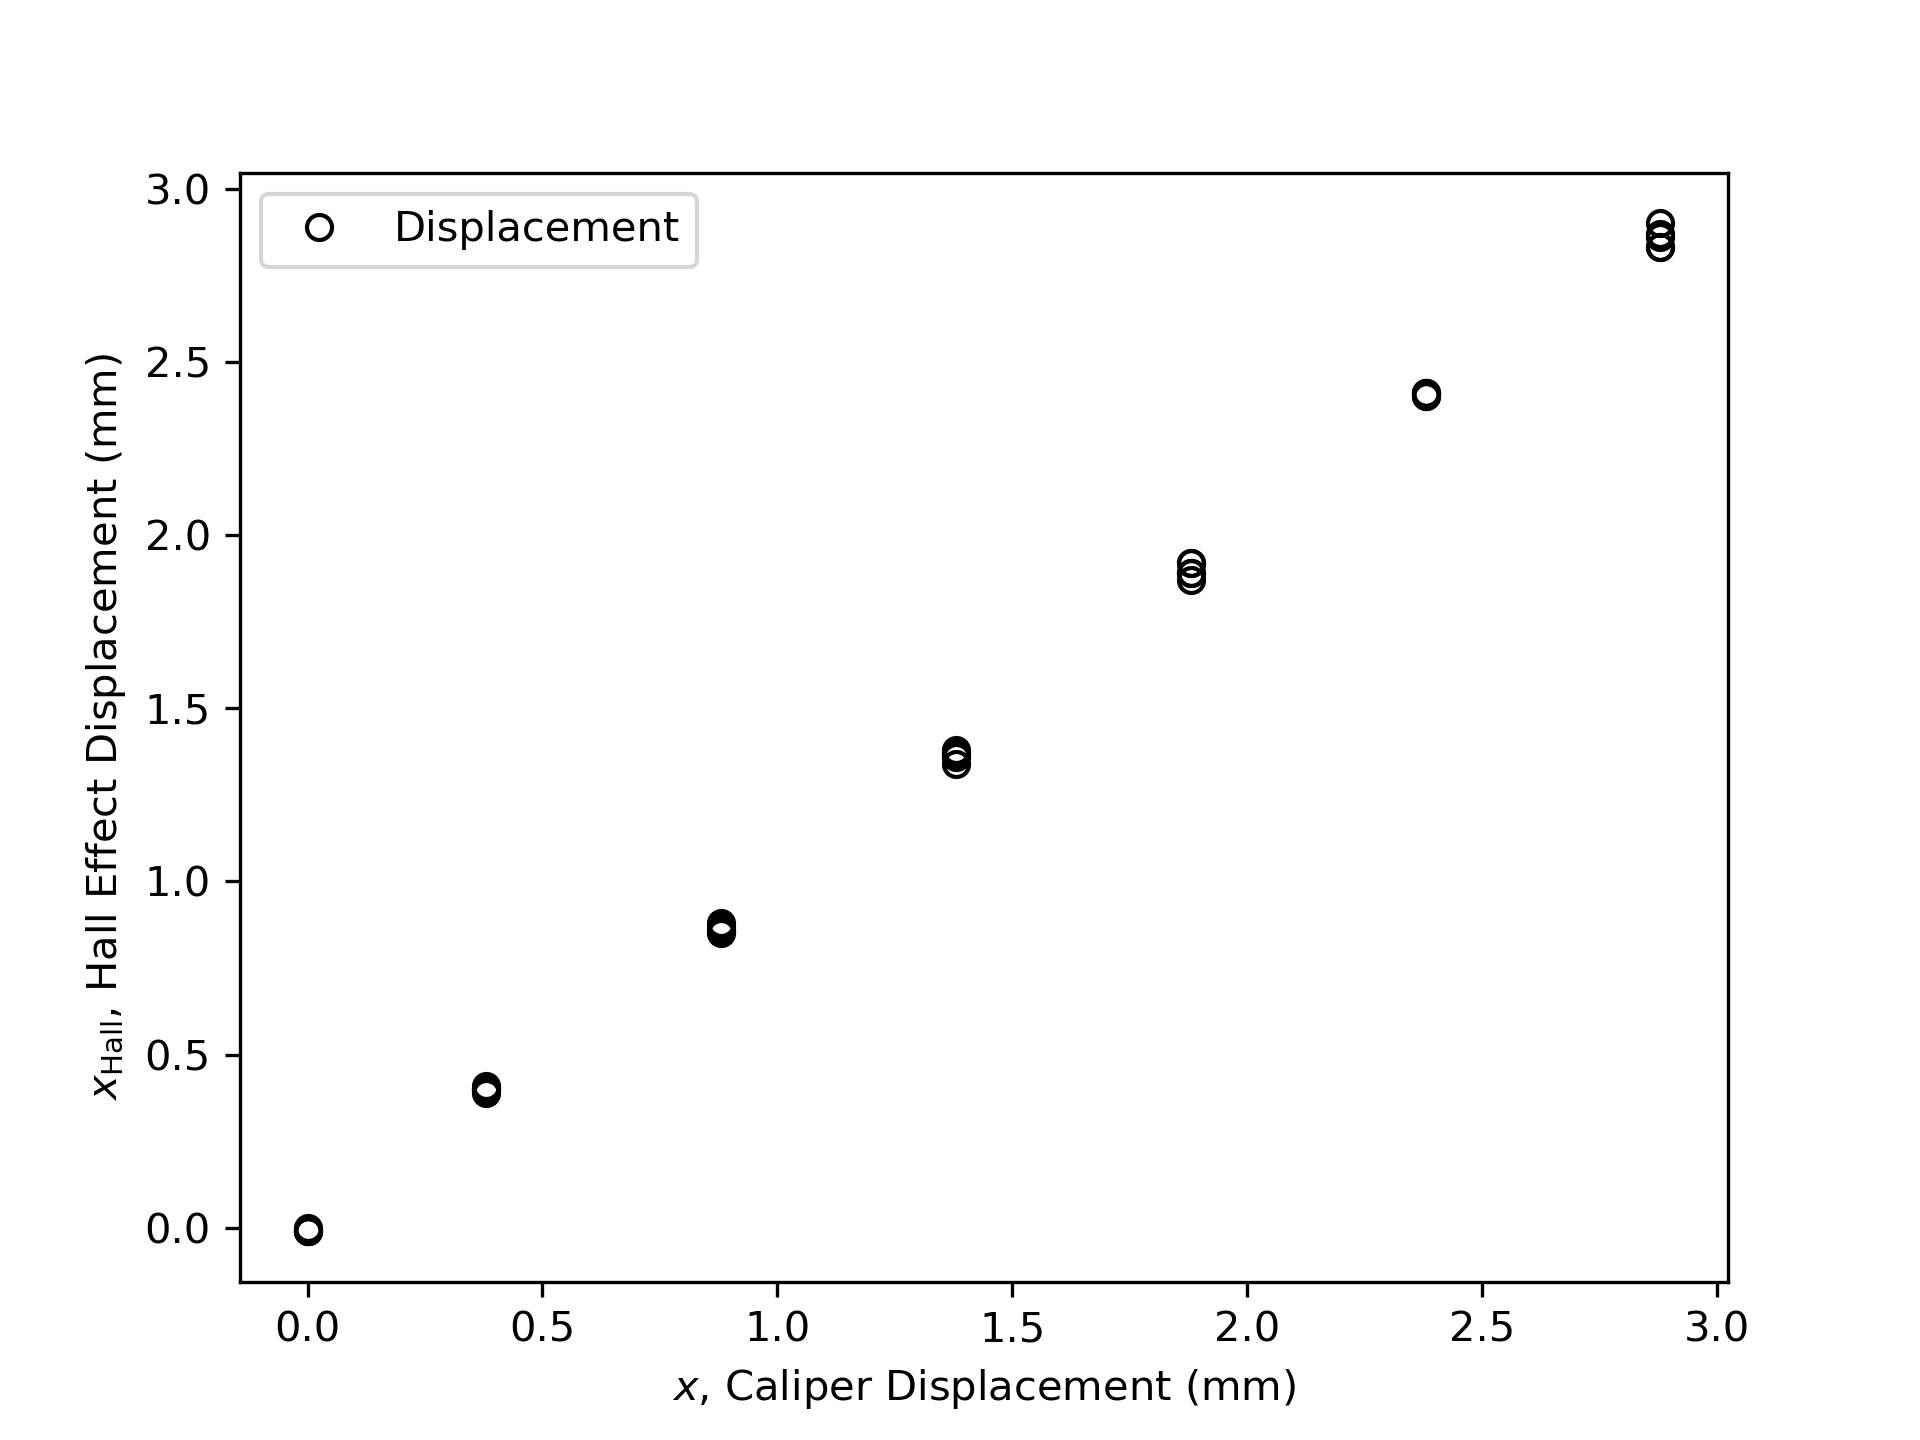
\includegraphics[width=0.8\linewidth]{matplotlib/Q2b.png}
    \caption{Hall-effect sensor displacement vs. caliper displacement}
    \label{fig:Q2b}
\end{figure}

A deviation of the Hall-effect sensor displacement from the caliper displacement was calculated. The deviation is shown in Table \ref{tab:Q2b}.

\begin{table}[h]
    \centering
    \caption{Deviation of Hall-effect sensor displacement from caliper displacement}
    \label{tab:Q2b}
    \begin{tabular}{cccccc}
        \hline
         & \multicolumn{5}{c}{Reading} \\
        \cline{2-6}
        Displacement & 1 & 2 & 3 & 4 & 5 \\
        \midrule
        (mm) & (mm) & (mm) & (mm) & (mm) & (mm) \\
        \midrule
        0.00 & -0.01 & -0.01 & 0.00 & -0.01 & -0.01 \\
        0.38 & 0.02 & 0.03 & 0.02 & 0.02 & 0.01 \\
        0.88 & -0.02 & 0.00 & -0.01 & -0.02 & -0.03 \\
        1.38 & -0.02 & -0.04 & 0.00 & -0.01 & -0.01 \\
        1.88 & 0.04 & 0.04 & 0.01 & 0.01 & -0.01 \\
        2.38 & 0.02 & 0.03 & 0.03 & 0.03 & 0.02 \\
        2.88 & -0.05 & 0.02 & -0.01 & -0.05 & -0.02 \\
        \hline
    \end{tabular}
\end{table}

The accuracy of the Hall-effect sensor was found by taking the maximum of the absolute value of the deviations. 

\[
    \boxed{\text{Accuracy} = \max(|\text{Deviations}|) = 0.05 \;\; [\si[]{mm}]} 
\]

\FloatBarrier
\subsection{}
% c) The sensitivity of a non-linear correlating function is not constant with respect 
% to the input (i.e., sensitivity, !"
% !#
% , is a function of displacement). Find the sensitivity function
% by: i) plotting Hall-effect voltage (y-axis) vs caliper reading (x-axis), ii) fitting the data 
% with a third-order polynomial, and iii) taking the derivative of the polynomial. What is the 
% sensitivity when the displacement is zero? What is the sensitivity when the displacement 
% is 3 mm?

Repeating section a), with the Hall-effect voltage as the dependent variable and the caliper reading as the independent variable,
the coefficients of the polynomial of the form $y = ax^3 + bx^2 + cx + d$ were taken using the \texttt{=LINEST(x, y\string^\{1, 2, 3\}, True, True)}.
The plot of the Hall-effect voltage vs. caliper reading is shown in Fig. \ref{fig:Q2c}.

\begin{figure}[h]
    \centering
    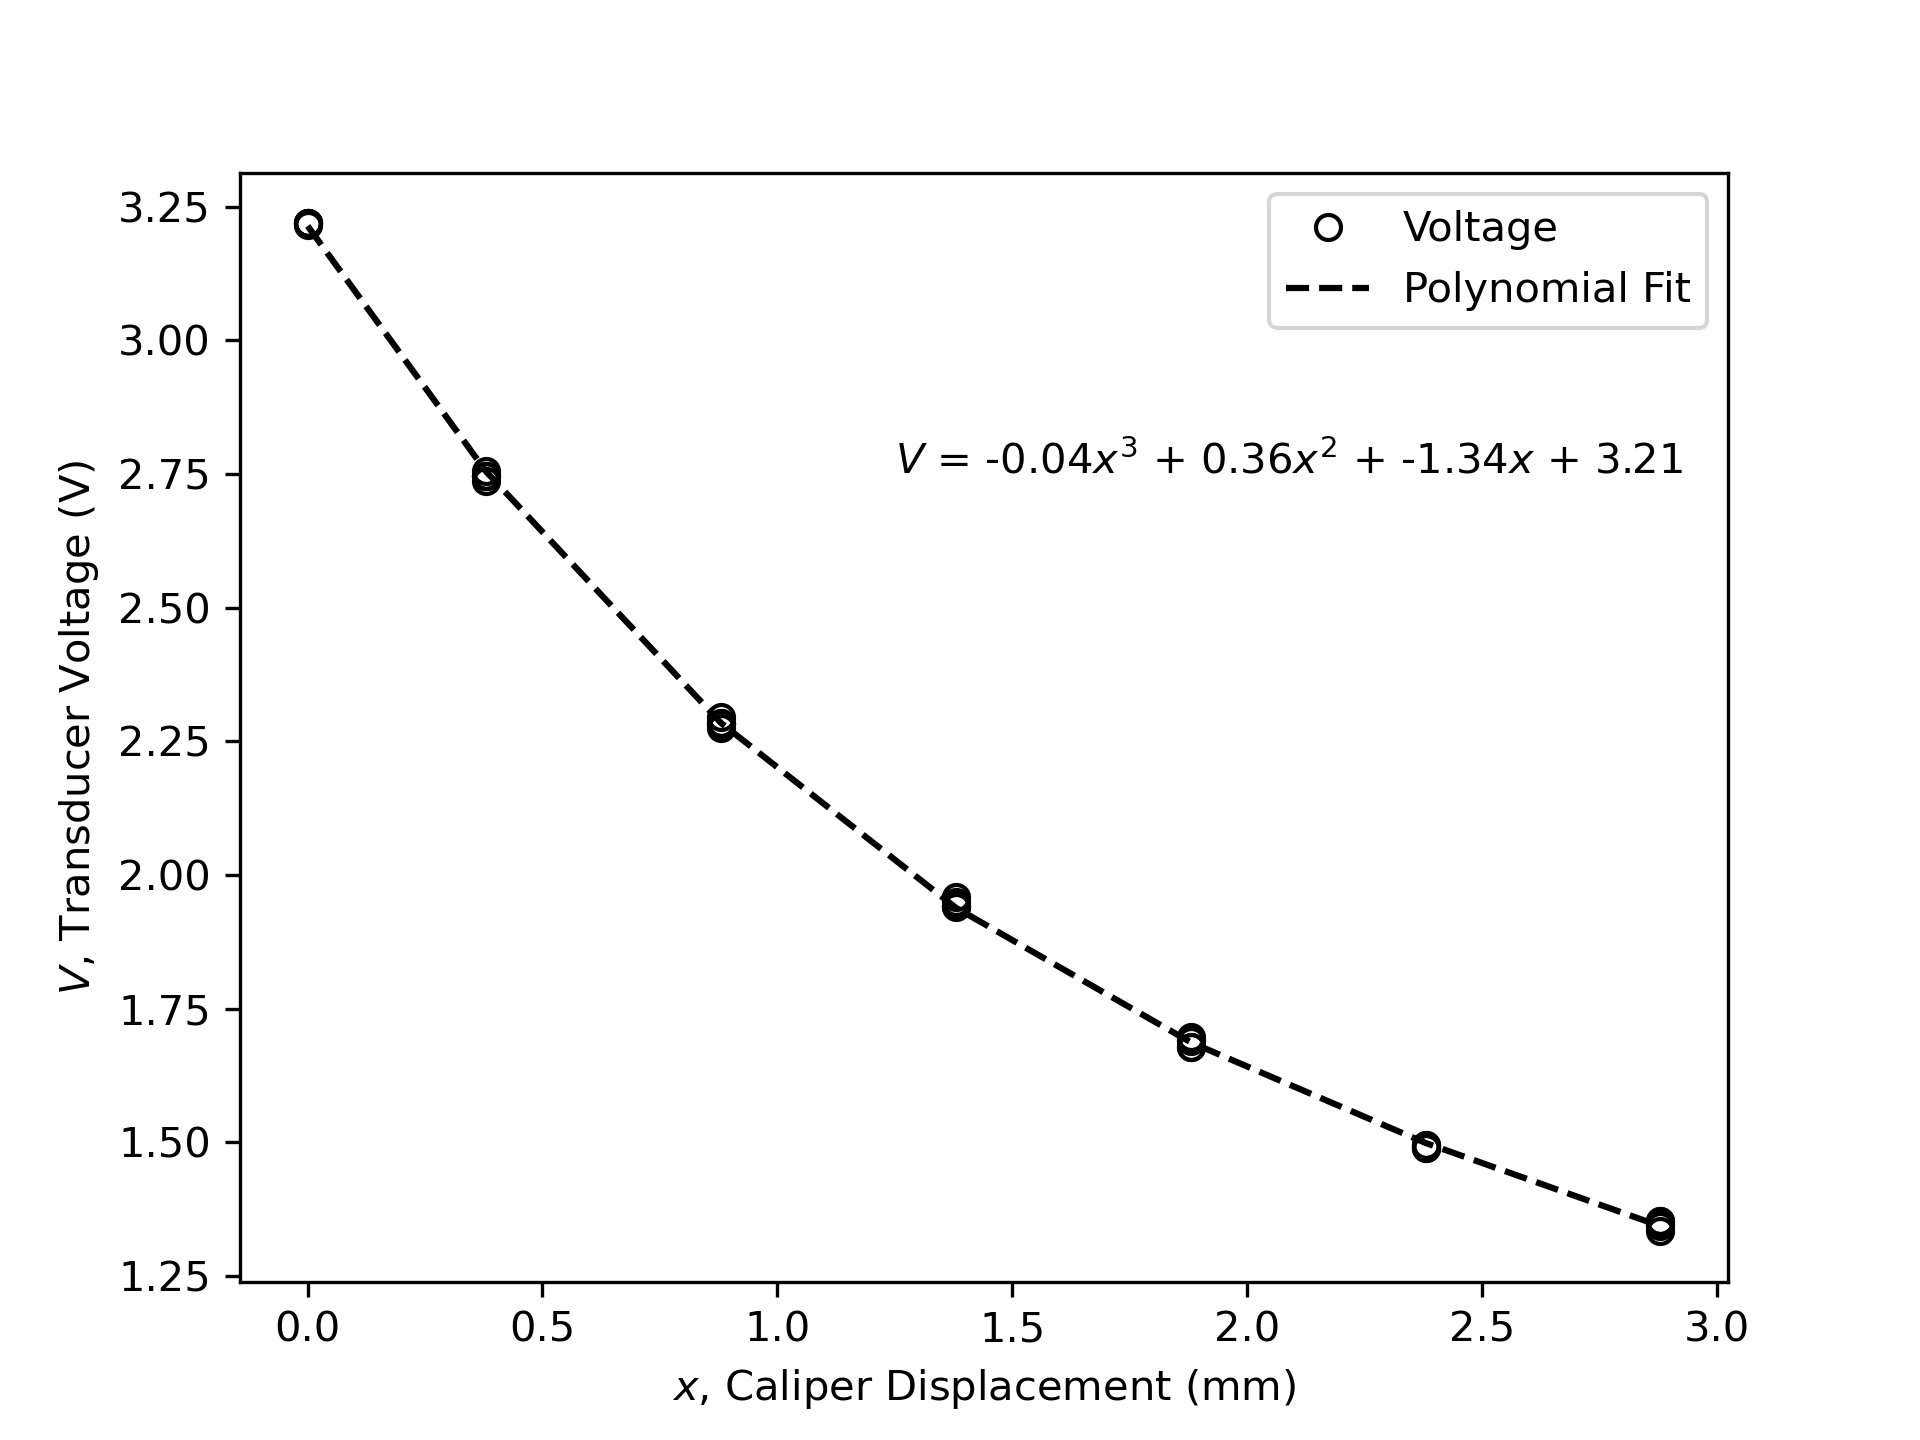
\includegraphics[width=0.8\linewidth]{matplotlib/Q2c.png}
    \caption{Hall-effect voltage vs. caliper reading}
    \label{fig:Q2c}
\end{figure}

The fit function is 
\begin{equation}
    V = -0.04x^3 + 0.36x^2 - 1.34x + 3.21 \;\; [\si[]{V}] \label{eq:Q2c}
\end{equation}

The derivative of Eq. (\ref{eq:Q2c}) is
\begin{equation}
    \frac{dV}{dx} = -0.12x^2 + 0.72x - 1.34 \;\; [\si[]{V/mm}] \label{eq:Q2c-derivative}
\end{equation}  

The sensitivity when the displacement is zero is
% \[
%     \boxed{\text{Sensitivity at } x = \qty{0}{mm} = -1.34 \;\; [\si[]{V/mm}]}
% \]

\[
  \boxed{\text{Sensitivity at } x = \qty{0}{mm} = \qty{-1.34}{V/mm}}  
\]

The sensitivity when the displacement is 3mm is
% \[
%     \boxed{\text{Sensitivity at } x = \qty{3}{mm} = -0.30 \;\; [\si[]{V/mm}]}
% \]

\[
    \boxed{\text{Sensitivity at } x = \qty{3}{mm} = \qty{-0.30}{V/mm}}
\]

\FloatBarrier
\subsection{}
% d) Does the potentiometer or the Hall-effect sensor have the highest sensitivity? 
% Which would be better at measuring small displacements? Why?

The Hall-effect sensor has the highest sensitivity. The sensitivity of the Hall-effect sensor at 0 mm and 3 mm is -1.34 V/mm and -0.30 V/mm respectively, both
of which are higher than the sensitivity of the potentiometer at 0.07891 V/mm for all measurements in its span. 

The Hall-effect sensor would be better at measuring small displacements because it has a higher sensitivity. A small change in displacement would result in a larger
change in voltage, which would be easier to detect.